%%%%%%%%%%%%%%%%%%%%%%%%%%%%%%%%%%%%%%%%%
% Stylish Article
% LaTeX Template
% Version 2.1 (1/10/15)
%
% This template has been downloaded from:
% http://www.LaTeXTemplates.com
%
% Original author:
% Mathias Legrand (legrand.mathias@gmail.com) 
% With extensive modifications by:
% Vel (vel@latextemplates.com)
%
% Authors:
% Mauricio Hoyos Ardila mhoyosa2@eafit.edu.co
% Jonathan Zapata Castaño jzapat80@eafit.edu.co
%
% License:
% CC BY-NC-SA 3.0 (http://creativecommons.org/licenses/by-nc-sa/3.0/)
%
%%%%%%%%%%%%%%%%%%%%%%%%%%%%%%%%%%%%%%%%%

%----------------------------------------------------------------------------------------
%	PACKAGES AND OTHER DOCUMENT CONFIGURATIONS
%----------------------------------------------------------------------------------------

\documentclass[fleqn,10pt]{SelfArx} % Document font size and equations flushed left

\usepackage[english]{babel} % Specify a different language here - english by default

\usepackage{lipsum} % Required to insert dummy text. To be removed otherwise

%----------------------------------------------------------------------------------------
%	COLUMNS
%----------------------------------------------------------------------------------------

\setlength{\columnsep}{0.55cm} % Distance between the two columns of text
\setlength{\fboxrule}{0.75pt} % Width of the border around the abstract

%----------------------------------------------------------------------------------------
%	COLORS
%----------------------------------------------------------------------------------------

\definecolor{color1}{RGB}{0,0,0} % Color of the article title and sections
\definecolor{color2}{RGB}{0,20,20} % Color of the boxes behind the abstract and headings

%----------------------------------------------------------------------------------------
%	HYPERLINKS
%----------------------------------------------------------------------------------------

\usepackage{hyperref} % Required for hyperlinks
\hypersetup{hidelinks,colorlinks,breaklinks=true,urlcolor=color2,citecolor=color1,linkcolor=color1,bookmarksopen=false,pdftitle={Title},pdfauthor={Author}}

%----------------------------------------------------------------------------------------
%	ARTICLE INFORMATION
%----------------------------------------------------------------------------------------

\JournalInfo{Reporte Técnico, No. 1, 2017} % Journal information
\Archive{Universidad EAFIT} % Additional notes (e.g. copyright, DOI, review/research article)

\PaperTitle{Clústering de Documentos a partir de Métricas de Similitud} % Article title

\Authors{Mauricio Hoyos\textsuperscript{1}, Jonathan Zapata\textsuperscript{2}} % Authors
\affiliation{\textsuperscript{1}\textit{Departamento de Ingeniería de Sistemas, Universidad EAFIT, Medellín, Colombia, } \textbf{mhoyosa2@eafit.edu.co}} % Author affiliation
\affiliation{\textsuperscript{2}\textit{Departamento de Ingeniería de Sistemas, Universidad EAFIT, Medellín, Colombia, } \textbf{jzapat80@eafit.edu.co}} % Author affiliation

\Keywords{K-means --- Jacard --- MPI --- Cluster --- HPC --- Paralelización --- Particionamiento por dominio --- Similitud } % Keywords 

\newcommand{\keywordname}{Keywords} % Defines the keywords heading name

%----------------------------------------------------------------------------------------
%	ABSTRACT
%----------------------------------------------------------------------------------------

\Abstract{Text mining is an analysis technique which has allowed us to implement a set of new applications through the time. Such as search engines in the web (Google, Facebook, Amazon, Spotify, Netflix, among others), suggestions systems, natural language processing and others.
The document clustering techniques enable us to link a document with other similar documents according to a comparison metric.
The basic idea of the proposed implementations is to compare the efficiency between computing in a single node and computing in a distributed network of nodes.}

%----------------------------------------------------------------------------------------

\begin{document}

\flushbottom % Makes all text pages the same height

\maketitle % Print the title and abstract box

\tableofcontents % Print the contents section

\thispagestyle{empty} % Removes page numbering from the first page

%----------------------------------------------------------------------------------------
%	ARTICLE CONTENTS
%----------------------------------------------------------------------------------------

\section*{Introducción} % The \section*{} command stops section numbering

\addcontentsline{toc}{section}{Introducción} % Adds this section to the table of contents

Actualmente, debido a la gran cantidad de información que se encuentra en los medios, y a que está alojada en diferentes bases de datos, surge la necesidad de agrupar dicha información en un conjunto de datos que permita realizar búsquedas más rápidas, para ello se  crearon técnicas que permiten calcular la similitud que tienen dos textos; una de las más utilizadas es la minería de datos, la cual, como su nombre lo indica, se encarga de extraer las partes importantes de un archivo (en nuestro caso un texto). El enfoque que le dimos al proyecto está delimitado precisamente por esta área de la ciencia de datos, la cual nos va a permitir crear varios set de documentos y determinar el número de sets apropiados para agrupar la información, esto gracias a diferentes experimentos, además de generar un informe detallado evaluando el contraste (figura \ref{fig:graficoSerialParalelo}) de compartamientos entre el tiempo de ejecución del programa en serial y el paralelo con diferentes datasets.

En este caso, decidimos hacer que la agrupación de documentos sea mediante el uso de los algoritmos k-means y Jaccard, estos son el principal soporte para determinar la similitud entre documentos.
 
%------------------------------------------------

\section{Marco Teórico}

\subsection{Descripción del Problema}

%\begin{enumerate}[noitemsep] % [noitemsep] removes whitespace between the items for a compact look
%\item First item in a list
%\item Second item in a list
%\item Third item in a list
%\end{enumerate}


\begin{description}
	\item[Document Clustering] Is the act of collecting similar documents into bins, where similarity is some function on a document. \ref{refer:1}
	\item[K-means Algorithm] Explanation
	\item[Jaccard Algorithm] Text \ref{refer:1}
\end{description}

%\begin{itemize}[noitemsep] % [noitemsep] removes whitespace between the items for a compact look
%	\item First item in a list
%	\item Second item in a list
%	\item Third item in a list
%\end{itemize}

%\subsubsection{Subsubsection}

\begin{figure*}[ht]\centering % Using \begin{figure*} makes the figure take up the entire width of the page
	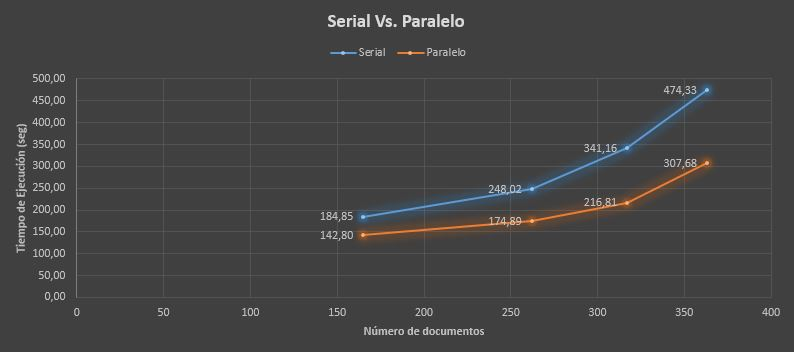
\includegraphics[width=\linewidth]{graficoSerialParalelo}
	\caption{Gráfico Serial Vs. Paralelo}
	\label{fig:graficoSerialParalelo}
\end{figure*}

%------------------------------------------------

\section{Análisis y Diseño (PCAM)}

\subsection{Análisis y Diseño:}

\paragraph{Particionamiento:}
Esta característica fue tenida en cuenta en el momento de realizar el conteo de palabras ya que cada nodo puede realizarlo sobre un grupo diferente de datos sin depender del conteo de los demás nodos. 
De esta misma manera se emplea el particionamiento al realizar el conteo de las palabras más importantes seleccionadas  mediante los cálculos previos.
Este puede ser considerado un buen particionamiento ya que divide tanto los cálculos asociados con el problema como los datos sobre los cuales opera.

\paragraph{Comunicación:}
El proceso de comunicación es de vital importancia, ya que nos permite obtener los datos que requiere cada nodo para realizar las funciones que le fueron encargadas, esta fase de comunicación se puede evidenciar cuando se hacen operaciones de lectura y escritura de datos que se encuentran en otros nodos, en este caso hace falta la aplicación de dicha técnica.


\paragraph{Aglomeración:}
Los algoritmos empleados para determinar la similitud y comparación de diferentes textos necesita juntar toda la información procesada por los nodos, así que dicha información es aglomerada en un solo nodo para la ejecucion de instrucciones de naturaleza serial, este tipo de fase en la que se recurre a la separación y recolección de datos, es la que más aplicamos en el transcurso de toda la ejecución.

\paragraph{Mapeo:}
La tecnología nos permite fácilmente repartir tareas entre los diferentes nodos, independientemente del número que haya, por lo que garantizamos mapeo al asignar una tarea al número de nodos que le asignamos a la ejecución del programa. Cada tarea es asignada a un procesador, en nuestro caso aplicamos mucho el concepto SIMD.

Los algoritmos que usamos están descritos en el marco teórico, pues son técnicas ampliamente probadas.
Las estructuras de datos que usamos son las fundamentales (int, bool, char[], matrices, etc), diccionarios y listas.
En cuanto al rendimiento análitico de la solución se puede encontrar que es de orden cúbico.


\section{Implementación}

A continuación compartimos nuestro trabajo a todo aquel que quiera evidenciar el análisis presentado en este estudio: https://github.com/jonyzp/HPC

\section{Análisis de resultados (secuencial vs. paralelo)}

A continuación presentamos el gráfico resultante del proceso de medición, el cual evidencia las aceleraciones entre datasets e implementaciones y en distintas ejecuciones.

\begin{table}[hbt]
	\caption{Tabla de Comparaciones de tiempo}
	\centering
	\begin{tabular}{llr}
%		\toprule
%		\multicolumn{1}{c}{Parámetro de comparación} \\
		\cmidrule(r){1-3}
		SetSize (MB) & T. Serial (seg) & T. Paralelo (seg)\\
		\midrule
		
		119,92 & 474,33 & 307,68 \\
		
		94,88 & 341,16 & 216,81 \\
		
		75,02 & 248,02 & 174,89 \\
		
		68,66 & 184,85 & 142,80 \\
		
		\bottomrule
	\end{tabular}
	\label{tab:label}
\end{table}


Se puede evidenciar la diferencia entre ejecutar el algoritmo de forma paralela a ejecutarlo de manera serial, aunque el algoritmo paralelo tiene un mayor orden de complejidad, logra reducir el tiempo que tarda en dar la solución, ya que el procesamiento se realiza de una manera distribuída




%------------------------------------------------
\phantomsection
\section*{Conclusiones} % The \section*{} command stops section numbering

\addcontentsline{toc}{section}{Acknowledgments} % Adds this section to the table of contents

\begin{itemize}
	\item Hay que saber atacar adecuadamente el problema para identificar qué procesos son los que se pueden optimizar por medio del procesamiento en co-paralelo
	\item Debido al tipo de dato que se estaba manejando en el procesamiento de los nodos es difícil optimizar pensando en la fase de la aglomeración de los datos.
	\item Es de anotar que no siempre se da por sentado que antes de resolver un problema hay que sentarse a diseñar primero, por lo que no sobra mencionar la importancia de tener al lado una hoja y un lápiz.
	\item La manera de estructurar un algoritmo serial comparada con la del paralelo cambia, precisamente para facilitar la paralelización, o en ocasiones, porque representa un limitante de implementación.
\end{itemize}
% So long and thanks for all the fish \cite{Figueredo:2009dg}.

%----------------------------------------------------------------------------------------
%	REFERENCE LIST
%----------------------------------------------------------------------------------------
\phantomsection
\bibliographystyle{unsrt}
%\bibliography{sample}

\begin{itemize}[noitemsep] % [noitemsep] removes whitespace between the items for a compact look
	\item DISEÑO DE ALGORITMOS PARALELOS
	En el texto: (cs.buap, 2017)
	Bibliografía: cs.buap. (2017). Diseño de algoritmos paralelos. 
	
	[online] Available at: https://www.cs.buap.mx/~mtovar/doc/ProgConc/ProgramacionParalela.pdf 
	
	[Accessed 21 Oct. 2017].
	\item cs.fit.edu. (2017). \textit{A Comparison of Document Clustering Techniques.} [online] Available at: http://cs.fit.edu/~pkc/classes/ml-internet/papers/steinbach00tr.pdf [Accessed 18 Oct. 2017].
	\label{refer:1}
\end{itemize}


%----------------------------------------------------------------------------------------

\end{document}